\documentclass[]{article}
\usepackage{lmodern}
\usepackage{amssymb,amsmath}
\usepackage{ifxetex,ifluatex}
\usepackage{fixltx2e} % provides \textsubscript
\ifnum 0\ifxetex 1\fi\ifluatex 1\fi=0 % if pdftex
  \usepackage[T1]{fontenc}
  \usepackage[utf8]{inputenc}
\else % if luatex or xelatex
  \ifxetex
    \usepackage{mathspec}
  \else
    \usepackage{fontspec}
  \fi
  \defaultfontfeatures{Ligatures=TeX,Scale=MatchLowercase}
\fi
% use upquote if available, for straight quotes in verbatim environments
\IfFileExists{upquote.sty}{\usepackage{upquote}}{}
% use microtype if available
\IfFileExists{microtype.sty}{%
\usepackage{microtype}
\UseMicrotypeSet[protrusion]{basicmath} % disable protrusion for tt fonts
}{}
\usepackage[margin=1in]{geometry}
\usepackage{hyperref}
\hypersetup{unicode=true,
            pdftitle={Predicting Gender from Risk-Seeking Behaviors},
            pdfauthor={Deepika Dilip, Rachel Tsong, and Adina Zhang},
            pdfborder={0 0 0},
            breaklinks=true}
\urlstyle{same}  % don't use monospace font for urls
\usepackage{color}
\usepackage{fancyvrb}
\newcommand{\VerbBar}{|}
\newcommand{\VERB}{\Verb[commandchars=\\\{\}]}
\DefineVerbatimEnvironment{Highlighting}{Verbatim}{commandchars=\\\{\}}
% Add ',fontsize=\small' for more characters per line
\usepackage{framed}
\definecolor{shadecolor}{RGB}{248,248,248}
\newenvironment{Shaded}{\begin{snugshade}}{\end{snugshade}}
\newcommand{\KeywordTok}[1]{\textcolor[rgb]{0.13,0.29,0.53}{\textbf{#1}}}
\newcommand{\DataTypeTok}[1]{\textcolor[rgb]{0.13,0.29,0.53}{#1}}
\newcommand{\DecValTok}[1]{\textcolor[rgb]{0.00,0.00,0.81}{#1}}
\newcommand{\BaseNTok}[1]{\textcolor[rgb]{0.00,0.00,0.81}{#1}}
\newcommand{\FloatTok}[1]{\textcolor[rgb]{0.00,0.00,0.81}{#1}}
\newcommand{\ConstantTok}[1]{\textcolor[rgb]{0.00,0.00,0.00}{#1}}
\newcommand{\CharTok}[1]{\textcolor[rgb]{0.31,0.60,0.02}{#1}}
\newcommand{\SpecialCharTok}[1]{\textcolor[rgb]{0.00,0.00,0.00}{#1}}
\newcommand{\StringTok}[1]{\textcolor[rgb]{0.31,0.60,0.02}{#1}}
\newcommand{\VerbatimStringTok}[1]{\textcolor[rgb]{0.31,0.60,0.02}{#1}}
\newcommand{\SpecialStringTok}[1]{\textcolor[rgb]{0.31,0.60,0.02}{#1}}
\newcommand{\ImportTok}[1]{#1}
\newcommand{\CommentTok}[1]{\textcolor[rgb]{0.56,0.35,0.01}{\textit{#1}}}
\newcommand{\DocumentationTok}[1]{\textcolor[rgb]{0.56,0.35,0.01}{\textbf{\textit{#1}}}}
\newcommand{\AnnotationTok}[1]{\textcolor[rgb]{0.56,0.35,0.01}{\textbf{\textit{#1}}}}
\newcommand{\CommentVarTok}[1]{\textcolor[rgb]{0.56,0.35,0.01}{\textbf{\textit{#1}}}}
\newcommand{\OtherTok}[1]{\textcolor[rgb]{0.56,0.35,0.01}{#1}}
\newcommand{\FunctionTok}[1]{\textcolor[rgb]{0.00,0.00,0.00}{#1}}
\newcommand{\VariableTok}[1]{\textcolor[rgb]{0.00,0.00,0.00}{#1}}
\newcommand{\ControlFlowTok}[1]{\textcolor[rgb]{0.13,0.29,0.53}{\textbf{#1}}}
\newcommand{\OperatorTok}[1]{\textcolor[rgb]{0.81,0.36,0.00}{\textbf{#1}}}
\newcommand{\BuiltInTok}[1]{#1}
\newcommand{\ExtensionTok}[1]{#1}
\newcommand{\PreprocessorTok}[1]{\textcolor[rgb]{0.56,0.35,0.01}{\textit{#1}}}
\newcommand{\AttributeTok}[1]{\textcolor[rgb]{0.77,0.63,0.00}{#1}}
\newcommand{\RegionMarkerTok}[1]{#1}
\newcommand{\InformationTok}[1]{\textcolor[rgb]{0.56,0.35,0.01}{\textbf{\textit{#1}}}}
\newcommand{\WarningTok}[1]{\textcolor[rgb]{0.56,0.35,0.01}{\textbf{\textit{#1}}}}
\newcommand{\AlertTok}[1]{\textcolor[rgb]{0.94,0.16,0.16}{#1}}
\newcommand{\ErrorTok}[1]{\textcolor[rgb]{0.64,0.00,0.00}{\textbf{#1}}}
\newcommand{\NormalTok}[1]{#1}
\usepackage{longtable,booktabs}
\usepackage{graphicx,grffile}
\makeatletter
\def\maxwidth{\ifdim\Gin@nat@width>\linewidth\linewidth\else\Gin@nat@width\fi}
\def\maxheight{\ifdim\Gin@nat@height>\textheight\textheight\else\Gin@nat@height\fi}
\makeatother
% Scale images if necessary, so that they will not overflow the page
% margins by default, and it is still possible to overwrite the defaults
% using explicit options in \includegraphics[width, height, ...]{}
\setkeys{Gin}{width=\maxwidth,height=\maxheight,keepaspectratio}
\IfFileExists{parskip.sty}{%
\usepackage{parskip}
}{% else
\setlength{\parindent}{0pt}
\setlength{\parskip}{6pt plus 2pt minus 1pt}
}
\setlength{\emergencystretch}{3em}  % prevent overfull lines
\providecommand{\tightlist}{%
  \setlength{\itemsep}{0pt}\setlength{\parskip}{0pt}}
\setcounter{secnumdepth}{0}
% Redefines (sub)paragraphs to behave more like sections
\ifx\paragraph\undefined\else
\let\oldparagraph\paragraph
\renewcommand{\paragraph}[1]{\oldparagraph{#1}\mbox{}}
\fi
\ifx\subparagraph\undefined\else
\let\oldsubparagraph\subparagraph
\renewcommand{\subparagraph}[1]{\oldsubparagraph{#1}\mbox{}}
\fi

%%% Use protect on footnotes to avoid problems with footnotes in titles
\let\rmarkdownfootnote\footnote%
\def\footnote{\protect\rmarkdownfootnote}

%%% Change title format to be more compact
\usepackage{titling}

% Create subtitle command for use in maketitle
\providecommand{\subtitle}[1]{
  \posttitle{
    \begin{center}\large#1\end{center}
    }
}

\setlength{\droptitle}{-2em}

  \title{Predicting Gender from Risk-Seeking Behaviors}
    \pretitle{\vspace{\droptitle}\centering\huge}
  \posttitle{\par}
    \author{Deepika Dilip, Rachel Tsong, and Adina Zhang}
    \preauthor{\centering\large\emph}
  \postauthor{\par}
      \predate{\centering\large\emph}
  \postdate{\par}
    \date{May 14, 2019}


\begin{document}
\maketitle

\subsection{Introduction}\label{introduction}

One public health phenomenon that has been the subject of debate is the
``Gender and Health Paradox'', in which women experience decreased
quality of life, yet have higher life expectancies than men. A theory
that seeks to explain this pattern outlines increased risk-taking by men
as a causal mechanism. By this logic, men would indicate more
risk-taking behaviors than women when controlled for age and other
confounders. We sought to test this theory by examining if risk-seeking
behaviors could be predictive of gender.

\textbf{Young People's Survey}

For our analysis, we used a data set consisting of 1,010 responses from
a 2013 survey administered among statistics students and their friends
at Comenius University in Bratislava, Slovakia. This dataset is
available to download from Kaggle. The survey consisted of 150 items
including music and movie preferences, hobbies and interests, phobias,
health habits, personality traits, views on life, and opinions, spending
habits, and demographics. Most of the items were presented as a
five-point Likert scale indicating how much a respondent agreed to the
statement. Participants were given the survey in both electronic and
paper formats. To test our hypotheses, we selected 19 variables that
would demonstrate risk-seeking behavior.

After sectioning the data accordingly, we counted missing values to
determine if that could affect our results. When only completed
responses were considered (i.e.~having values for every variable), we
had a sample size of 942; 6.7\% of the data was missing. As this value
was less than 10\%, we decided not to address this via imputation and
opted for a deletion method (complete-case analysis). The limitations of
this method will be addressed in the discussion.

\subsection{Data Exploration}\label{data-exploration}

We checked for collinearity of variables via a correlation matrix; as
there were no significant correlations between any predictors, all of
our original variables were retained. We stratified responses by gender
and visualized them in histograms (fig. 1). Some predictors have more
skewed distributions by gender compared to others (e.g.~cars, war
movies). Other variables such as alcohol use and going outdoors were
more evenly distributed by gender.

We used an unsupervised learning technique (principle component
analysis) to further explore the data (fig. 2). Due to the large number
of predictors, the first and second components only explained 17.1\% and
9.4\% of the total variance in the data respectively. Nevertheless, PCA
was insightful in that some of the variables mostly explained by the
first component (interest in cars, adrenaline-driven sports, and active
sports) were skewed toward males.

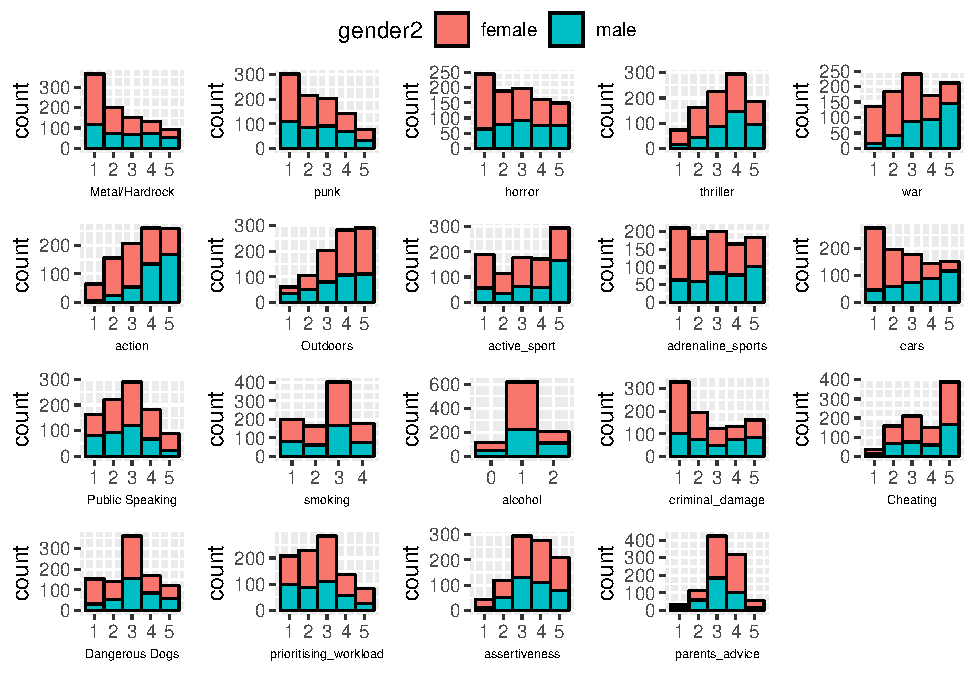
\includegraphics{final_report_files/figure-latex/unnamed-chunk-1-1.pdf}
\textbf{Figure 1: Variable Distributions by Gender}

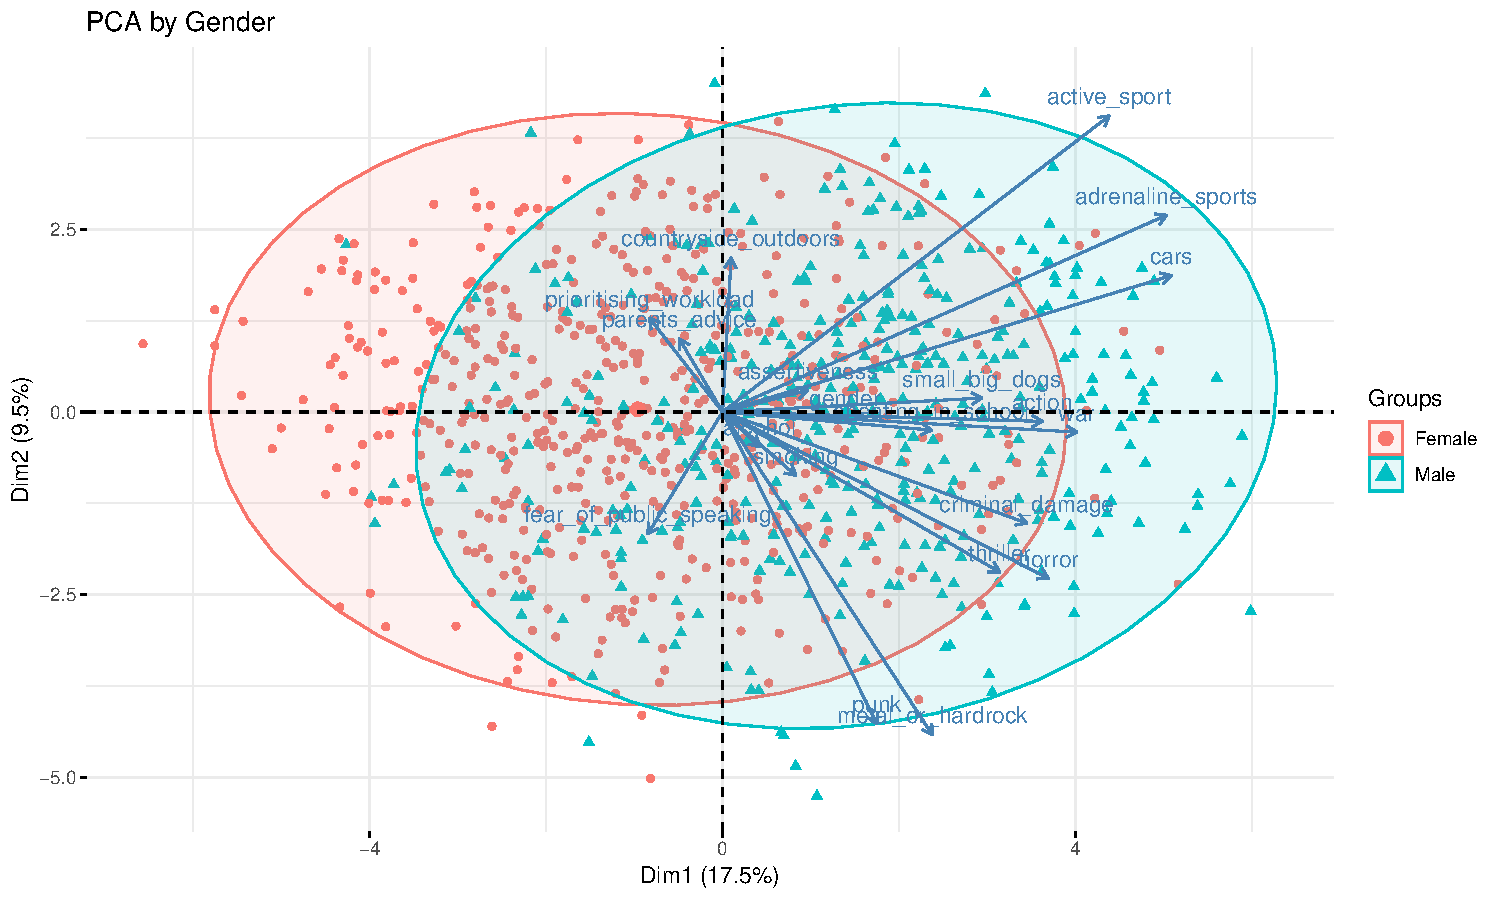
\includegraphics{final_report_files/figure-latex/unnamed-chunk-2-1.pdf}
\textbf{Figure 2: PCA}

\subsection{Method}\label{method}

We selected 19 variables that were related to thrill or risk seeking
behaviors. The following variables were included in our analysis:

\begin{itemize}
\item
  Interest in: (ranked 1-5 from ``don't enjoy at all'' to ``enjoy very
  much'')

  \begin{itemize}
  \tightlist
  \item
    Metal, hard rock music
  \item
    Punk music
  \item
    Horror movies
  \item
    War movies
  \item
    Action movies
  \item
    Outdoor activities
  \item
    Sport at a competitive level
  \item
    Adrenaline sports
  \item
    Cars
  \end{itemize}
\item
  Fears of public speaking (ranked 1-5 from ``not afraid at all'' to
  ``very afraid of'')
\item
  Smoking habits (categorical with 4 levels: ``never smoked'', ``tried
  smoking'', ``former smoker'', ``current smoker'')
\item
  Drinking habits (categorical with 3 levels: ``never'', ``social
  drinker'', ``drink a lot'')
\item
  Statements about personality traits: (ranked 1-5 from ``strongly
  disagree'' to ``strongly agree'')

  \begin{itemize}
  \tightlist
  \item
    I damaged things in the past when I get angry
  \item
    I used to cheat at school
  \item
    I prefer big dangerous dogs to smaller, calmer dogs
  \item
    I try to do tasks as soon as possible and not leave them until last
    minute
  \item
    I'm not afraid to give my opinion if I feel strongly about something
  \item
    I always listen to my parents' advice
  \end{itemize}
\end{itemize}

Variables that were ranked on a scale from 1-5 were considered as
continous responses. After splitting the data into training and testing
sets using an 80/20 split, we fit the following models to the training
data:

\begin{itemize}
\tightlist
\item
  Logistic regression
\item
  Discriminant analysis (linear and quadratic)
\item
  KNN
\item
  Support vector machine (linear and radial kernels)
\item
  Classification trees (random forest and boosting)
\end{itemize}

Training and test error were calculated for each model to evaluate
overfitting. The final model was chosen by assessing the training data
using the \texttt{resamples()} function in the \texttt{caret} package.

\subsection{Models}\label{models}

\subsubsection{Logistic Regression}\label{logistic-regression}

Logistic regression assumes independent observations, a sufficiently
large sample size, and a linear relationship between the predictors and
the log-odds of the outcome. As we used simple logistic regression, via
the \texttt{caret} package, it does not contain any tuning parameters.
When examining the predictor parameters, the following variables had a
p-value of less than 0.001: \texttt{cars}, \texttt{war},
\texttt{action}, and \texttt{metal\_or\_hardrock}, indicating that these
are important predictors of gender.

\subsubsection{Discriminant Analysis}\label{discriminant-analysis}

\textbf{Linear}

For LDA, we used the \texttt{caret} package. Linear discriminant
analysis assumes normally distributed features. LDA does not contain any
tuning parameters and is strong when considering more than 2 predictors.
Additionally, it works well when the classes are well separated and
Gaussian distribution assumptions are applied. When ranking variables
(using the function \texttt{varImp()}), the most important ones were as
follows: \texttt{cars}, \texttt{war}, \texttt{action},
\texttt{active\_sport}, and \texttt{thriller}.

\textbf{Quadratic}

For QDA, we used the \texttt{caret} package. Just like LDA, QDA works
well when the classes are well separated and Gaussian distribution
(normally -distributed) assumptions are applied. However, unlike LDA, it
assumes that each class has its own covariance matrix. QDA does not
contain any tuning parameters. When ranking variables (using the
function varImp()), the most important ones were as follows:
\texttt{cars}, \texttt{war}, \texttt{action}, \texttt{active\_sport},
and \texttt{thriller}.

\subsubsection{KNN}\label{knn}

The method of K-nearest neighbors makes no assumptions about the shape
of the decision boundary; therefore, if the decision boundary is highly
non-linear then this model will perform better than others. This model
has one tuning parameter, K, the number of closest training points. An
optimal value of K was chosen by repeated cross-validation using the
\texttt{train()} function in the \texttt{caret} package by specifying
the tuning grid. THe optimal K was 94. One drawback of this model is
that we cannot assess variable importance.

\subsubsection{SVM}\label{svm}

\textbf{Linear}

The support vector classifier has one tuning parameter, C. Using the
\texttt{train()} function in the \texttt{caret} package the best C was
0.0433, which was chosen by cross-validation. Since the support vector
classifier is a hyperplane, the model assumes that the decision boundary
is linear, which is a potential drawback if the decision boundary is
non-linear.

\textbf{Radial}

The support vector machine with a radial kernel has two tuning
parameters. One is C, the cost parameter, and the other is the degree of
non-linearity sigma. We used the \texttt{train()} function in the
\texttt{caret} package to choose these parameters by cross-validation.
The best C was 78.033 and the best sigma was 0.000335. This model
assumes a non-linear boundary. One potential drawback of support vector
machines is that you cannot assess variable importance or estimate
probabilities as in logistic regression.

\subsubsection{Random Forest}\label{random-forest}

A Random Forest (RF) model was fit with the \texttt{caret} package using
the \texttt{ranger} method. We chose Random Forest as one of our models
because it is an ensemble method for classification trees that uses a
collection of models to improve the final prediction. Random Forest was
also chosen over bagging as an esemble method because it minimizes
correlation between the decisions trees that are grown. In our model,
500 decision trees were grown and the gini index was selected as a
splitrule. The minimum number of variables to randomly sample at each
split (mtry) and minimum node size were tuned using repeated
cross-validation in the \texttt{caret} packages with ROC as the measure
of performance. The best tuning results were \texttt{mtry\ =\ 2} and
\texttt{min.node.size\ =\ 6}. According to the final model, the most
important variables for classification are \texttt{cars},
\texttt{action}, and \texttt{war}.

\subsubsection{Extreme Gradient
Boosting}\label{extreme-gradient-boosting}

An Extreme Gradient Boosting (XGB) model was fit using the
\texttt{xgboost} packages in \texttt{caret}. Gradient Boosting is
another ensemble method for classification trees. It differs from other
ensemble methods such as random forest because the algorithm focuses on
modelling errors from previous models in order to improve the
bias-variance tradeoff. We selected the \texttt{xgboost} package and
algorithm because it performs more efficiently than the \texttt{gbm}
package discussed in class. Multiple parameters were tuned using
repeated cross-validation with ROC as the unit of measurement. The final
model selected \texttt{nrounds\ =\ 100}, \texttt{max\_depth\ =\ 2},
\texttt{eta\ =\ 0.1}, \texttt{colsample\_bytree\ =\ 0.8}. The final
model showed that \texttt{cars}, \texttt{action}, and \texttt{war} were
the most important variables for classifying gender.

\begin{longtable}[]{@{}lrr@{}}
\toprule
Models & TrainError & TestError\tabularnewline
\midrule
\endhead
Logistic & 0.2066225 & 0.2032086\tabularnewline
LDA & 0.2119205 & 0.1925134\tabularnewline
QDA & 0.1509934 & 0.2032086\tabularnewline
KNN & 0.2357616 & 0.2139037\tabularnewline
SVM Linear & 0.2119205 & 0.1818182\tabularnewline
SVM Radial & 0.2039735 & 0.1871658\tabularnewline
Random Forest & 0.0000000 & 0.1764706\tabularnewline
XGBoost & 0.1562914 & 0.1764706\tabularnewline
\bottomrule
\end{longtable}

Table 1: Testing and training error rates among eight classification
models

\subsection{Model Selection}\label{model-selection}

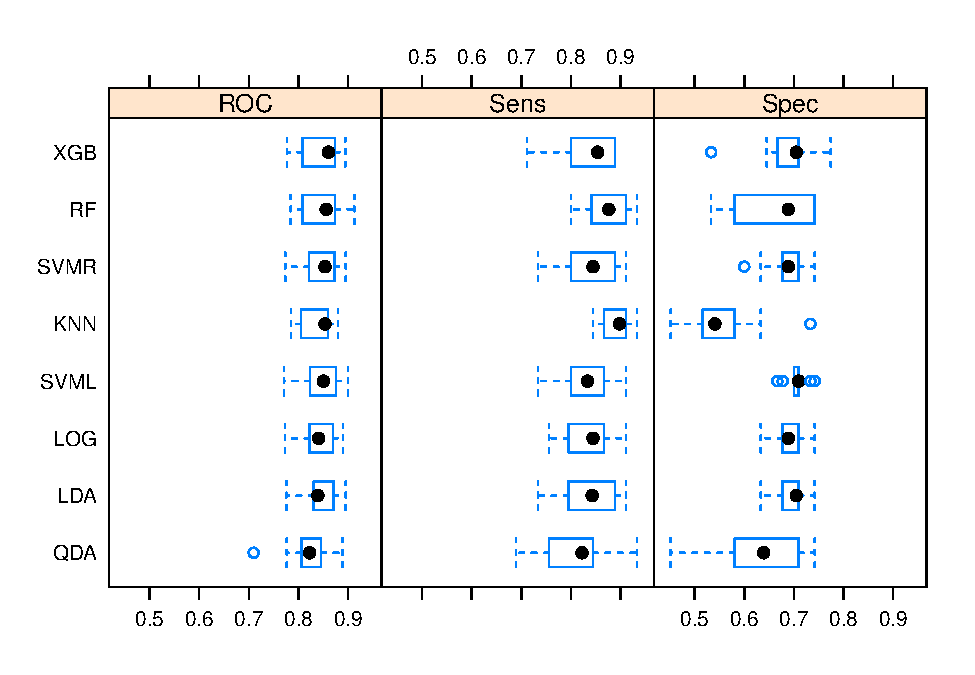
\includegraphics{final_report_files/figure-latex/unnamed-chunk-13-1.pdf}

\textbf{Figure 3: Comparison of Model Fits}

Each model was resampled through the \texttt{caret} package and the
results are shown in the figure above. Overall, all of our models fit
well with most ROC's ranging around 80\%. The sensitivity and
specificity measures have more variability and fall within a wider
range. XGBoost and Random Forest perform the best and they perform as
well as each other. The median ROC of XGBoost is higher while the means
are very similar. The median sensitivity of XGBoost is slightly lower
than Random Forest, but the median specificity of XGBoost is higher and
the interquartile range is narrower. On the other hand, QDA performed
the worst. The median and mean ROC were lowest as was sensitivity. While
QDA did not have the lowest specificity, the interquartile range is
wide.

\subsection{Final Model}\label{final-model}

Based off of our resampling results through the \texttt{caret} package,
we chose XGBoost as our final model. Althought this model performs as
well as random forest, we chose this model because it reported a higher
specificity. Although the random forest training error rate was 0\%, we
were concerned that this meant that the model overfit the data;
therefore, we chose XGBoost over the random forest. From XGBoost, the
most important variables for classifying individuals by gender were
based off their interest in cars, action movies, and war movies (fig.
3).

Even though we pick boosting for our a final model, there are
limitations to picking this method. A classification tree by itself is
very easy to interpret, however the use of ensemble methods utilizes
multiple trees making a final model more difficult to visualize or
interpret.

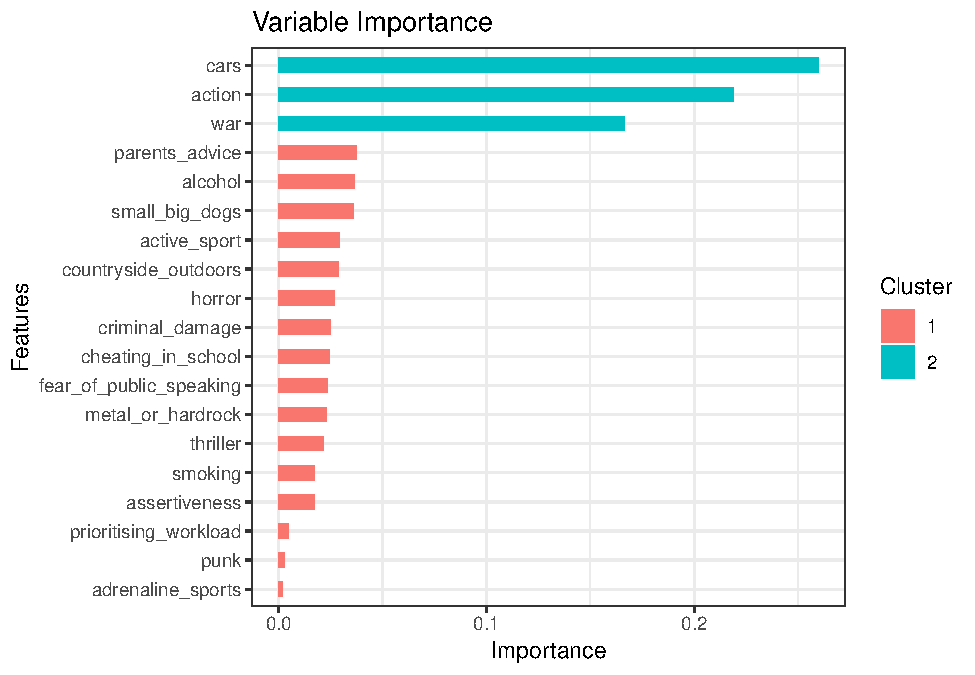
\includegraphics{final_report_files/figure-latex/unnamed-chunk-14-1.pdf}
\textbf{Figure 4: Variable Importance for Final Model}

\subsection{Conclusion}\label{conclusion}

The boosting model performed the best in terms of minimizing testing
error rates and increased accuracy (it had a testing error rate of 0.21,
mean AUC of 0.85, mean sensitivity of 0.84, and mean specificity of
0.71).

Our models were overall consistent regarding which predictors were more
indicative of gender. Most of them concerned interests in specific movie
genres or topics (e.g.~cars, action movies, war movies). Given that the
marketing of such genres are heavily gender-based, this is not
surprising. The most important variable among behaviors, according to
the boosting model, was taking parents' advice and alcohol intake, but
these were ranked below several variables concerning movie interests.

Our predictors lacked collinearity, but even for our simpler models
(i.e.~logistic regression), our model accuracies were higher than
expected. For context, the lowest mean AUC value was 0.83 from Quadratic
Discriminant Analysis, which, by rule of thumb, is a good classifier
performance.

One major finding was that interests were more predictive of gender in
comparison to behaviors and personalities. This supports the work of
sociologists that gender is learned and prescribed by social factors
rather than biologically inherited. While additional literature and
findings would be necessary for us to make solid conclusions, many of
our chosen predictors were suggestive of gender. This could speak to
gender roles and behaviors as a whole. Future analyses should include
more demographic information and a more diverse sample (in terms of
location/age/etc.) in order to yield more generalizable results.

\subsubsection{Limitations}\label{limitations}

Some of the limitations of this report include translation issues. The
original language of the survey was Slovakian, and this could influence
interpretations. Additionally, this affects generalizability of findings
as the population of this survey was specifically statistics students in
Slovakia. The deletion method used would also present issues if data
were not missing at random, resulting in bias.

\newpage

\subsection{Appendix}\label{appendix}

\subsubsection{Code}\label{code}

\begin{Shaded}
\begin{Highlighting}[]
\CommentTok{# libraries}
\KeywordTok{library}\NormalTok{(tidyverse)}
\KeywordTok{library}\NormalTok{(dplyr)}
\KeywordTok{library}\NormalTok{(caret)}
\KeywordTok{library}\NormalTok{(ranger)}
\KeywordTok{library}\NormalTok{(xgboost)}
\KeywordTok{library}\NormalTok{(pROC)}
\KeywordTok{library}\NormalTok{(factoextra)}
\KeywordTok{library}\NormalTok{(ggpubr)}
\KeywordTok{library}\NormalTok{(Ckmeans.1d.dp)}

\CommentTok{# Load Datset}
\NormalTok{dat1 =}\StringTok{ }\KeywordTok{read_csv}\NormalTok{(}\StringTok{"./final.csv"}\NormalTok{) }\OperatorTok
\StringTok{  }\NormalTok{dplyr}\OperatorTok{::}\KeywordTok{select}\NormalTok{(}\OperatorTok{-}\NormalTok{X1) }\OperatorTok
\StringTok{  }\KeywordTok{mutate}\NormalTok{(}\DataTypeTok{gender =} \KeywordTok{ifelse}\NormalTok{(gender }\OperatorTok{==}\StringTok{ }\DecValTok{0}\NormalTok{, }\StringTok{"female"}\NormalTok{, }\StringTok{"male"}\NormalTok{))}

\KeywordTok{set.seed}\NormalTok{(}\DecValTok{1}\NormalTok{)}
\CommentTok{# Partition dataset into training and testing datasets}
\NormalTok{row_train =}\StringTok{ }\KeywordTok{createDataPartition}\NormalTok{(}\DataTypeTok{y =}\NormalTok{ dat1}\OperatorTok{$}\NormalTok{gender, }\DataTypeTok{p =} \FloatTok{0.8}\NormalTok{, }\DataTypeTok{list =} \OtherTok{FALSE}\NormalTok{)}
\NormalTok{dat1_train =}\StringTok{ }\NormalTok{dat1[row_train,]}
\NormalTok{dat1_test =}\StringTok{ }\NormalTok{dat1[}\OperatorTok{-}\NormalTok{row_train,]}

\CommentTok{# Set up cross-validation for tuning parameters}
\NormalTok{ctrl =}\StringTok{ }\KeywordTok{trainControl}\NormalTok{(}\DataTypeTok{method =} \StringTok{"repeatedcv"}\NormalTok{,}
                    \DataTypeTok{summaryFunction =}\NormalTok{ twoClassSummary,}
                    \DataTypeTok{classProbs =} \OtherTok{TRUE}\NormalTok{)}

\KeywordTok{set.seed}\NormalTok{(}\DecValTok{1}\NormalTok{) }
\CommentTok{# Fit a logistic regression }
\NormalTok{log.fit =}\StringTok{ }\KeywordTok{train}\NormalTok{(gender}\OperatorTok{~}\NormalTok{., dat1_train,}
                 \DataTypeTok{method =} \StringTok{"glm"}\NormalTok{,}
                 \DataTypeTok{metric =} \StringTok{"ROC"}\NormalTok{,}
                 \DataTypeTok{trControl =}\NormalTok{ ctrl)}

\CommentTok{# Fit LDA model}
\NormalTok{lda.fit =}\StringTok{ }\KeywordTok{train}\NormalTok{(gender}\OperatorTok{~}\NormalTok{., dat1_train, }
                   \DataTypeTok{method =} \StringTok{"lda"}\NormalTok{, }
                   \DataTypeTok{metric =} \StringTok{"ROC"}\NormalTok{, }
                   \DataTypeTok{trControl =}\NormalTok{ ctrl)}
\CommentTok{# Fit QDA model}
\NormalTok{qda.fit <-}\StringTok{ }\KeywordTok{train}\NormalTok{(gender}\OperatorTok{~}\NormalTok{., dat1_train, }
                   \DataTypeTok{method =} \StringTok{"qda"}\NormalTok{, }
                   \DataTypeTok{metric =} \StringTok{"ROC"}\NormalTok{, }
                   \DataTypeTok{trControl =}\NormalTok{ ctrl)}
\CommentTok{# fit KNN}
\NormalTok{knn.fit =}\StringTok{ }\KeywordTok{train}\NormalTok{(}\DataTypeTok{x =}\NormalTok{ dat1_train[,}\DecValTok{1}\OperatorTok{:}\DecValTok{19}\NormalTok{],}
                \DataTypeTok{y =}\NormalTok{ dat1_train}\OperatorTok{$}\NormalTok{gender,}
                \DataTypeTok{method =} \StringTok{"knn"}\NormalTok{,}
                \DataTypeTok{preProcess =} \KeywordTok{c}\NormalTok{(}\StringTok{"center"}\NormalTok{, }\StringTok{"scale"}\NormalTok{),}
                \DataTypeTok{tuneGrid =} \KeywordTok{data.frame}\NormalTok{(}\DataTypeTok{k =} \KeywordTok{seq}\NormalTok{(}\DecValTok{50}\NormalTok{, }\DecValTok{120}\NormalTok{, }\DataTypeTok{by =} \DecValTok{2}\NormalTok{)),}
                \DataTypeTok{trControl =}\NormalTok{ ctrl)}
\CommentTok{# Run linear SVM}
\NormalTok{svm_linear =}\StringTok{ }\KeywordTok{train}\NormalTok{(gender }\OperatorTok{~}\StringTok{ }\NormalTok{. ,}
                   \DataTypeTok{data =}\NormalTok{ dat1_train,}
                   \DataTypeTok{method =} \StringTok{"svmLinear2"}\NormalTok{,}
                   \DataTypeTok{preProcess =} \KeywordTok{c}\NormalTok{(}\StringTok{"center"}\NormalTok{, }\StringTok{"scale"}\NormalTok{),}
                   \DataTypeTok{tuneGrid =} \KeywordTok{data.frame}\NormalTok{(}\DataTypeTok{cost =} \KeywordTok{exp}\NormalTok{(}\KeywordTok{seq}\NormalTok{(}\OperatorTok{-}\DecValTok{5}\NormalTok{, }\DecValTok{1}\NormalTok{, }\DataTypeTok{len =} \DecValTok{30}\NormalTok{))),}
                   \DataTypeTok{metric =} \StringTok{"ROC"}\NormalTok{,}
                   \DataTypeTok{trControl =}\NormalTok{ ctrl)}
\CommentTok{# Set tuning grid}
\NormalTok{radial_grid =}\StringTok{ }\KeywordTok{expand.grid}\NormalTok{(}\DataTypeTok{C =} \KeywordTok{exp}\NormalTok{(}\KeywordTok{seq}\NormalTok{(}\OperatorTok{-}\DecValTok{4}\NormalTok{, }\DecValTok{5}\NormalTok{, }\DataTypeTok{len =} \DecValTok{15}\NormalTok{)),}
                          \DataTypeTok{sigma =} \KeywordTok{exp}\NormalTok{(}\KeywordTok{seq}\NormalTok{(}\OperatorTok{-}\DecValTok{8}\NormalTok{, }\OperatorTok{-}\DecValTok{5}\NormalTok{, }\DataTypeTok{len =} \DecValTok{5}\NormalTok{)))}

\CommentTok{# Fit radial SVM model}
\NormalTok{svm_radial =}\StringTok{ }\KeywordTok{train}\NormalTok{(gender }\OperatorTok{~}\StringTok{ }\NormalTok{.,}
                   \DataTypeTok{data =}\NormalTok{ dat1_train,}
                   \DataTypeTok{method =} \StringTok{"svmRadial"}\NormalTok{,}
                   \DataTypeTok{preProcess =} \KeywordTok{c}\NormalTok{(}\StringTok{"center"}\NormalTok{, }\StringTok{"scale"}\NormalTok{),}
                   \DataTypeTok{tuneGrid =}\NormalTok{ radial_grid,}
                   \DataTypeTok{metric =} \StringTok{"ROC"}\NormalTok{,}
                   \DataTypeTok{trControl =}\NormalTok{ ctrl)}
\CommentTok{# Set up tuning grid for random forest}
\NormalTok{rf.grid =}\StringTok{ }\KeywordTok{expand.grid}\NormalTok{(}\DataTypeTok{mtry =} \KeywordTok{seq}\NormalTok{(}\DataTypeTok{from =} \DecValTok{2}\NormalTok{, }\DataTypeTok{to =} \DecValTok{6}\NormalTok{, }\DataTypeTok{length.out =} \DecValTok{5}\NormalTok{),}
                      \DataTypeTok{splitrule =} \StringTok{"gini"}\NormalTok{,}
                      \DataTypeTok{min.node.size =} \DecValTok{1}\OperatorTok{:}\DecValTok{10}\NormalTok{)}

\CommentTok{# Run Random Forest}
\NormalTok{rf.fit =}\StringTok{ }\KeywordTok{train}\NormalTok{(gender}\OperatorTok{~}\NormalTok{., dat1_train,}
               \DataTypeTok{method =} \StringTok{"ranger"}\NormalTok{,}
               \DataTypeTok{tuneGrid =}\NormalTok{ rf.grid, }
               \DataTypeTok{trControl =}\NormalTok{ ctrl,}
               \DataTypeTok{metric =} \StringTok{"ROC"}\NormalTok{,}
               \DataTypeTok{importance =} \StringTok{"impurity"}\NormalTok{)}
\CommentTok{# set tuning grid}
\NormalTok{xgbGrid =}\StringTok{ }\KeywordTok{expand.grid}\NormalTok{(}\DataTypeTok{nrounds =} \KeywordTok{seq}\NormalTok{(}\DataTypeTok{from =} \DecValTok{50}\NormalTok{, }\DataTypeTok{to =} \DecValTok{200}\NormalTok{, }\DataTypeTok{by =} \DecValTok{50}\NormalTok{),  }
                      \DataTypeTok{max_depth =} \KeywordTok{c}\NormalTok{(}\DecValTok{2}\NormalTok{, }\DecValTok{3}\NormalTok{, }\DecValTok{4}\NormalTok{, }\DecValTok{5}\NormalTok{, }\DecValTok{6}\NormalTok{),}
                      \DataTypeTok{colsample_bytree =} \KeywordTok{seq}\NormalTok{(}\FloatTok{0.5}\NormalTok{, }\FloatTok{0.9}\NormalTok{, }\DataTypeTok{length.out =} \DecValTok{5}\NormalTok{),}
                      \DataTypeTok{eta =} \FloatTok{0.1}\NormalTok{,}
                      \DataTypeTok{gamma =} \DecValTok{0}\NormalTok{,}
                      \DataTypeTok{min_child_weight =} \DecValTok{1}\NormalTok{,}
                      \DataTypeTok{subsample =} \DecValTok{1}\NormalTok{)}

\CommentTok{# Run boosting model using xgboost method}
\NormalTok{xgb.fit =}\StringTok{ }\KeywordTok{train}\NormalTok{(gender}\OperatorTok{~}\NormalTok{., dat1_train,}
                \DataTypeTok{trControl =}\NormalTok{ ctrl,}
                \DataTypeTok{tuneGrid =}\NormalTok{ xgbGrid, }
                \DataTypeTok{method =} \StringTok{"xgbTree"}\NormalTok{,}
                \DataTypeTok{metric =} \StringTok{"ROC"}\NormalTok{,}
                \DataTypeTok{importance =} \StringTok{"impurity"}\NormalTok{)}

\CommentTok{# compare models using resamples()}
\NormalTok{resamp =}\StringTok{ }\KeywordTok{resamples}\NormalTok{(}\KeywordTok{list}\NormalTok{(}\DataTypeTok{LOG =}\NormalTok{ log.fit, }\DataTypeTok{LDA =}\NormalTok{ lda.fit,}
                        \DataTypeTok{QDA =}\NormalTok{ qda.fit, }\DataTypeTok{KNN =}\NormalTok{ knn.fit,}
                        \DataTypeTok{SVML =}\NormalTok{ svm_linear, }\DataTypeTok{SVMR =}\NormalTok{ svm_radial,}
                        \DataTypeTok{RF =}\NormalTok{ rf.fit, }\DataTypeTok{XGB =}\NormalTok{ xgb.fit))}
\KeywordTok{bwplot}\NormalTok{(resamp)}
\end{Highlighting}
\end{Shaded}

\textbf{Random forest mtry tuning results}
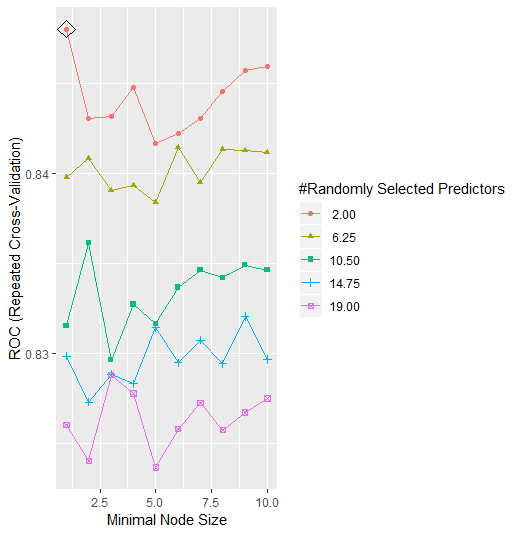
\includegraphics{rf_mtry_tune.png}

\textbf{XG Boost tuning results}

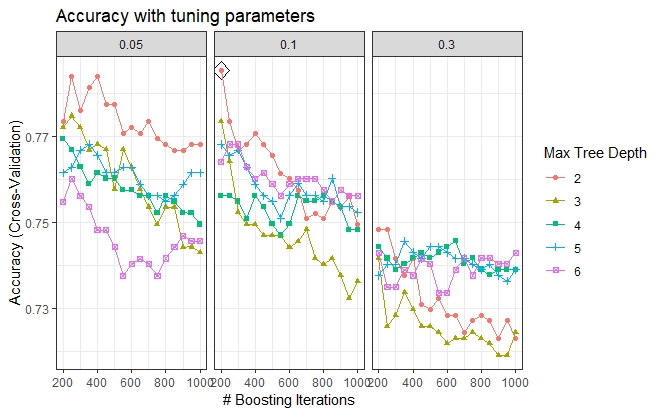
\includegraphics[width=9.19in]{tuning1_boost}
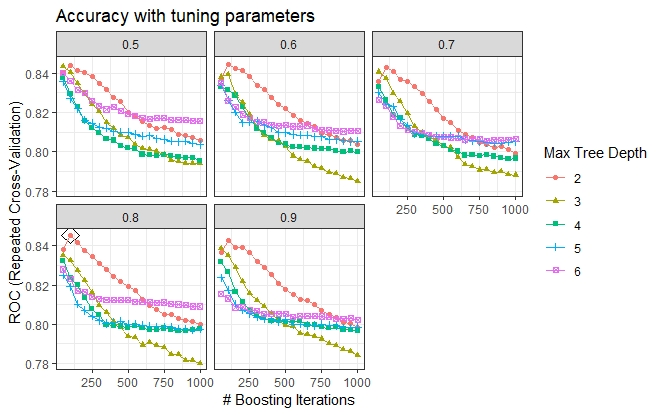
\includegraphics[width=9.19in]{tuning_performance}


\end{document}
